\chapter{PATTERN CREAZIONALI}

Questa tipologia di pattern \textit{astrae} il processo di creazione degli oggetti, fornendo diversi modi per associare un’interfaccia (o classe astratta) con 
un’implementazione e assicura che il programma sia scritto in termini di interfacce e non di implementazione.

\section{Perchè?}

Dal DIP sappiamo che è fondamentale non riferirsi a classi concrete (ma a classi astratte) e questo implica che ogni istruzione "new" mette a rischio questo principio.

Però, prima o poi, lo statement "new" deve essere usato ed è fondamentale che questo avvenga in poche e limitate parti del programma su cui abbiamo il controllo di 
flessibilità.

Se volessimo cambiare il tipo degli oggetti creati, saremmo in grado di farlo in un solo punto e senza troppe conseguenze al resto del programma.

\section{Factory Method}

Definisce un’interfaccia per creare un oggetto di un certo tipo ma lascia decidere alle sottoclassi quale oggetto istanziare.

La creazione di un'instanza avviene in un metodo (Factory method) che può essere astratto per poi essere implementato dalle sottoclassi oppure concreto per poi 
essere ridefinito dalle sottoclassi.

L'assegnazione dell'instanza viene salvata in una variabile, sempre nella classe base, privata e chi implementa/estende l'interfaccia/classe astratta avrà il compito 
di implementare/ridefinire il factory method.

Nella classe base il metodo restituirà il tipo dell'interfaccia desiderata, mentre nelle sottoclassi possiamo sfruttare la covarianza.

Nell'esempio di Application e Document, visto nel Template Method, il metodo createDocument() è il nostro factory method, infatti risulta essere astratto.

Factory Method serve a \textit{“parametrizzare”} rispetto alla creazione di un oggetto, basandosi solo su inheritance, ridefinizione di metodo e binding dinamico.

Se il linguaggio permettesse di passare un blocco di codice (lambda) che crea un oggetto, si potrebbe anche fare a meno di questo pattern ma non si parlerebbe più
di FactoryMethod.

\subsection{Struttura}
\begin{figure}[H]
    \centering
    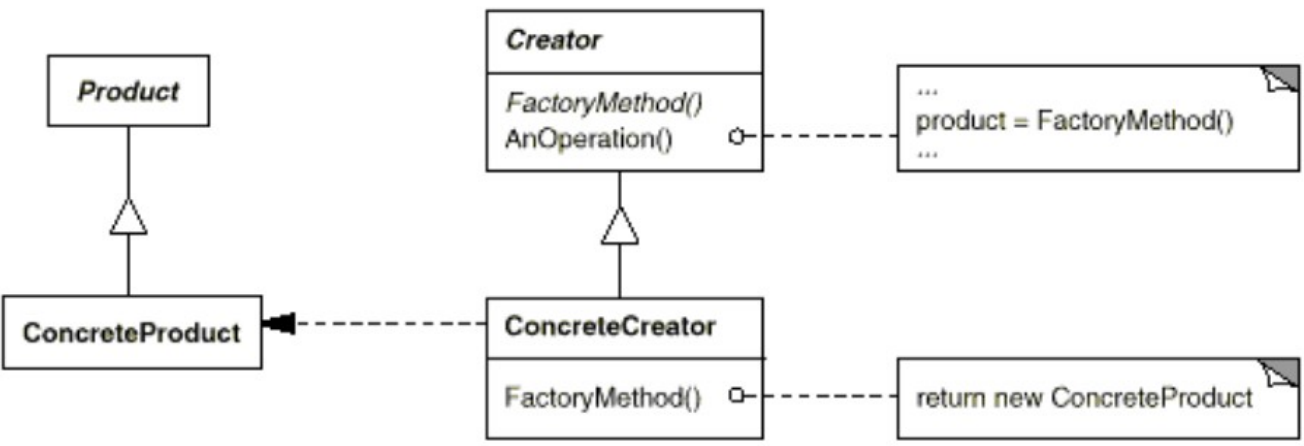
\includegraphics[width=0.5\linewidth]{pattern_creazionale/struttura_factory_method}
\end{figure}

\textbf{Product} definisce l'interfaccia degli oggetti creati tramite il FactoryMethod di Creator;

\textbf{Creator} dichiara il FactoryMethod, che restituisce un Product, con eventualmente un'implementazione di default, e lo chiama;

\textbf{ConcreteProduct} implementa l'interfaccia Product;

\textbf{ConcreteCreator} implementa o ridefinisce il FactoryMethod di Creator ritornando un ConcreteProduct.

\subsection{Factory Method vs Template Method}

Il factory method è un metodo, eventualmente \textit{astratto} e \textit{protetto}, che verrà poi implementato o ridefinito dalle sottoclassi e viene 
\textit{richiamato} da diversi metodi concreti della classe base ed è pensato per essere \textit{chiamato solo dalla classe base} (che lo dichiara).
\smallskip

Il template method è un metodo \textit{concreto}, eventualmete \textit{final}, che \textit{richiama} operazioni implementate da sottoclassi ed è pensato 
per essere \textit{chiamato dai client}

\subsection{Principale utilizzo}

Separare la creazione degli oggetti dal loro uso permette di modificare la loro creazione in modo consistente senza produrre una cascata di modifiche nel codice che 
li usa.

Molto usato nei framework, che generalmente esistono a livello astratto e non dovrebbero conoscere il tipo concreto degli oggetti da istanziare, questa responsabilità 
è lasciata al Client del framework, che provvederà a estendere il framework con sottoclassi per definire concretamente i factory methods.

Nell'esempio del Template Method, Application e Document sono la parte astratta del framework che si occupa di creare e gestire il framework, mentre la parte bassa 
è il Client che ridefinisce/implementa, a suo piacimento, i metodi.

\subsection{Vantaggi e svantaggi}

Con questo pattern si elimina la necessità di legare il codice di un’applicazione a classi concrete, il codice lavora con Product, quindi può lavorare con ogni specifico
prodotto definito dall’utente.
\smallskip

In compenso, siamo obbligati a creare una sottoclasse di Creator per creare una certa sottoclasse di Product (alternativa è quella di usare le lambda). 

Nel costruttore passiamo l'interfaccia funzionale Supplier e usiamo il suo metodo astratto, get(), nei metodi in cui assegnamo l'istanza.

Nel costruttore passiamo la lambda o sfruttiamo la method reference.

\begin{multicols}{2}
\begin{lstlisting}
public class Client {
    private MyType f;
    private Supplier<MyType> myTypeSupplier;
    
    public Client(Supplier<MyType> myTypeSupplier) {
        this.myTypeSupplier = myTypeSupplier;
    }
    public void init() {
        f = myTypeSupplier.get();
    }
    public void m() {
        f.n();
    }
    public void reset() {
        f = myTypeSupplier.get();
    }
}
\end{lstlisting}           
\columnbreak
\begin{lstlisting}
Client baseClient = new Client(MyImpl::new);
Client derivedClient = new Client(MyOtherImpl::new);
\end{lstlisting}
\end{multicols}

\section{Abstract Factory}

Fornisce un’interfaccia per creare famiglie di prodotti correlati o dipendenti senza specificare le loro classi concrete.

Il Client non crea gli oggetti direttamente ma delega la loro creazione a un altro oggetto.

\subsection{Struttura}

\begin{figure}[H]
    \centering
    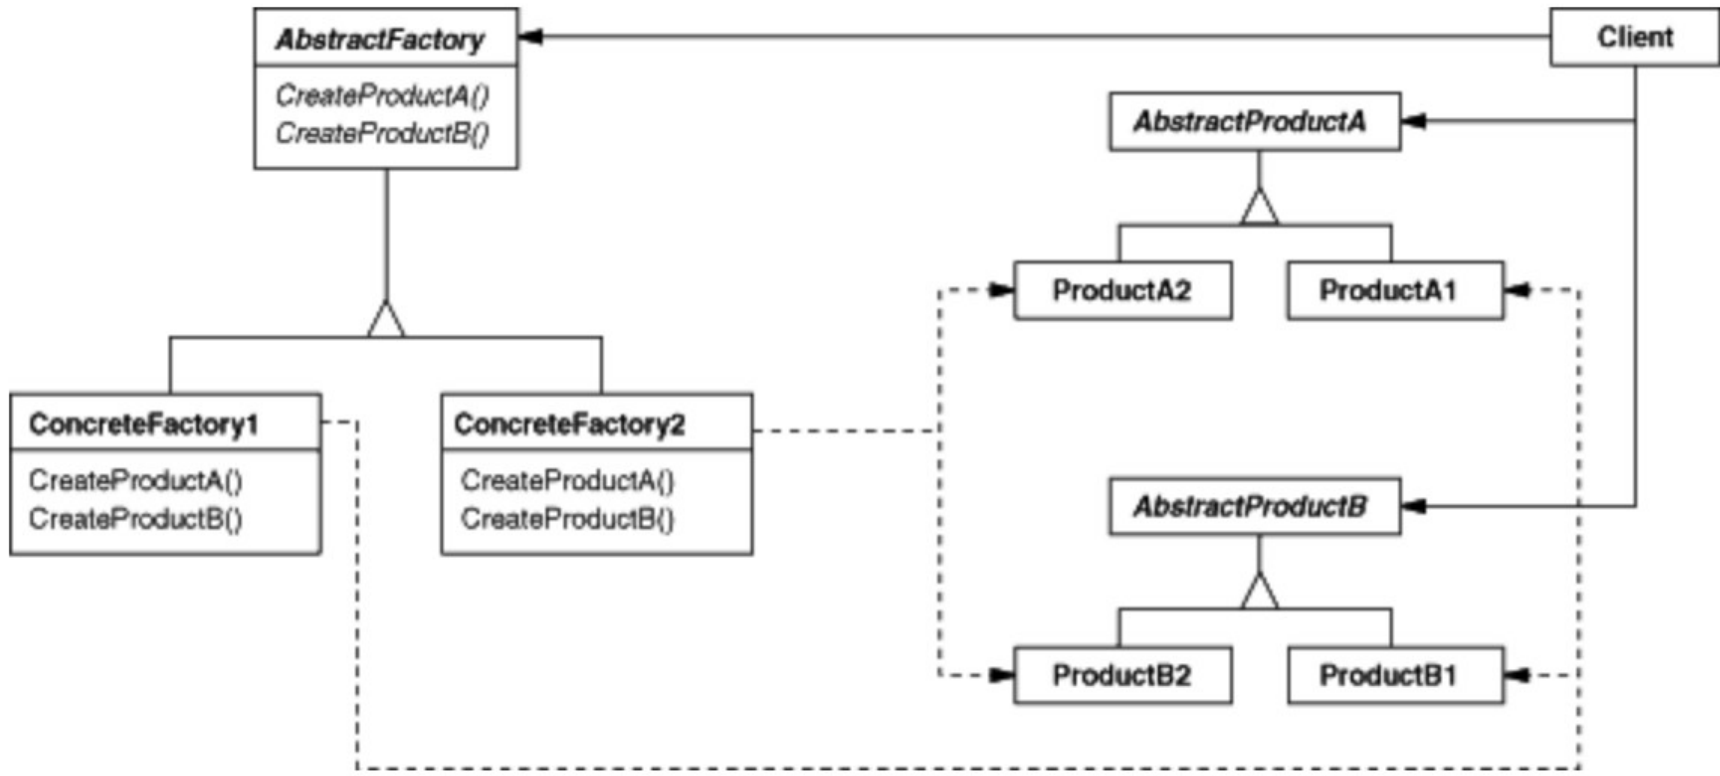
\includegraphics[width=0.5\linewidth]{pattern_creazionale/struttura_abstract_factory}
\end{figure}

\textbf{AbstractFactory} dichiara un’interfaccia per le operazioni di creazione di famiglie di AbstractProduct;

\textbf{AbstractProduct} interfaccia di una singola famiglia di prodotti;

\textbf{ConcreteFactory} implementa le operazioni per creare prodotti della stessa famiglia di un AbstractProduct;

\textbf{Product} implementazione di AbstractProduct.

\textbf{Client} utilizza l'AbstractFactory per la creazione di AbstractProduct.
\medskip

A run-time avremo una singola ConcreteFactory che crea, in modo consistente, una famiglia di prodotti.

\subsection{Conseguenze}

Se volessimo creare un'altra tipologia di prodotti, allora dovremmo istanziare ed usare un'altro tipo di ConcreteFactory, ogni famiglia di prodotti ha una propria 
implementazione di abstract factory.

Se si volesse aggiungere un nuovo prodotto, bisognerebbe aggiungere un nuovo metodo all'abstractFactory che sarà poi implementato dalle ConcretFactory.

\subsection{Principale utilizzo}

Un sistema deve essere indipendente da come gli oggetti sono creati, composti e rappresentati.

Un sistema che deve essere configurabile con una di tante famiglie di prodotti dove, i prodotti correlati di una stessa famiglia, sono progettati per essere usati 
insieme.

Si vuole fornire una libreria di oggetti rivelando solo le loro interfacce e non le loro implementazioni.

In quest'ultimo caso, le classi concrete dei prodotti, possono essere rese inaccessibili ai client mettendole in un package private, accessibili solo al package della
factory, cosicchè le factory sono le uniche a poter instanziare le classi concrete (un'altra variante è quella di usare classi anonime o interne ma avremo codice meno
leggibile).

\subsection{Accedere e modificare la factory}

Per accedere alla factory ci sono due alternative, esiste una sola instanza della factory (tramite uso del Singleton) oppure viene passata ai client attraverso un 
costruttore o setter.

Cambiare la factory a run-time può essere pericoloso in quanto, dopo il cambiamento, bisognerebbe notificare tutti i client in modo tale da ricreare tutti gli oggetti 
che sono stati instanziati attraverso la factory precedente.

Se la factory è implementata tramite Singleton, allora cambio l'instanza, se è implementata tramite setter, passo la nuova instanze oppure se è passata tramite 
costruttore, allora si ricreano le instanze dei client.

\subsection{AbstractFactory vs Factory Method}

Il primo è pensato per essere \textit{usato da altre classi} ed i suoi metodi sono \textit{pubblici}.

Il secondo è pensato per essere \textit{chiamato solo dalla classe base} (che lo dichiara) e \textit{non} deve essere pubblico.

\section{Static Factory Methods}

Sono un'alternativa alla creazione di oggetti con "new".

Dato un tipo MyType, invece di scrivere new MyType, scriveremo MyType.create dove il costruttore di MyType è reso privato e viene chiamato all'interno di un metodo 
statico di nome non necessariamente create.

A differenza dei costruttori, che sono vincolati ad avere lo stesso nome della classe e non ci possono essere più costruttori con la stessa firma, gli static factory 
method possono avere nomi più significativi.

Supponiamo di voler creare un oggetto TimeSpan specificando i secondi, minuti (entrambi interi).

Con i costruttori sarebbe più complicato perchè, anche cercando di usare l'overloading, avremo errore di compilazione in quanto avrebbero la stessa firma.

Quindi potremmo pensare di avere un unico costruttore, privato, che prende in input entrambi i parametri e creare quanti static factory method vogliamo, che ritornano
l'oggetto TimeSpan che fanno due cose differenti, uno per i secondi ed uno per i minuti.

\begin{lstlisting}
public class TimeSpan {
    private TimeSpan(int seconds, int minutes) {...}

    public static TimeSpan ofSeconds(int seconds) {
        return new TimeSpan(seconds, 0);
    }

    public static TimeSpan ofMinutes(int minutes) {
        return new TimeSpan(0, minutes);
    }
}
\end{lstlisting}

Se volessi creare un TimeSpan con le ore, basterebbe modificare il costruttore senza problemi, perchè privato, aggiungere le ore, creare un nuovo static factory method, 
chiamare al suo interno il nuovo costruttore e aggiornare gli static factory method esistenti.

\medskip
\textbf{N.B.} Se il construttore fosse stato pubblico, allora, dopo l'aggiunta del terzo parametro, avremmo avuto problemi di compilazione sia sul nostro codice che su 
quello dei client esterni.
\medskip

Quando si invoca un costruttore (tramite un "new") viene sempre creato un nuovo oggetto, con gli static factory methods, invece, si possono restituire oggetti condivisi.

\section{Singleton}

Assicurare che una classe abbia una sola istanza e ne fornisce un punto di accesso globale.

Viene implementato tramite uno static factory method (per convenzione si chiama getInstance) che restirtuisce l'instanzia in un campo statico privato 
(eventualmente crea l'oggetto la prima volta che viene chiamato).

\begin{lstlisting}
public class MyClass {
    private static MyClass instance = null;
    
    private MyClass() {...}

    public static MyClass getInstance() {
    if (instance == null) {
        instance = new MyClass();
    }
        return instance;
    }
}
\end{lstlisting}

\section{Fluent Interface}

Questo design pattern si basa sul Method Chaining, ovvero ogni metodo ritorna un oggetto, in modo da concatenare insieme tante invocazioni in un singolo statement, 
senza dover salvare i risultati intermedi in variabili locali.

Viene usato per fare il design delle API Object-Oriented, quindi tipico delle librerie e dei framework.

Un tipico caso d’uso è rimpiazzare i setter per rendere la configurazione di un oggetto più facile.

\section{Builder}

Separa la costruzione di un oggetto complesso dalla sua rappresentazione, la configurazione non viene fatta nel costruttore ma viene gestita da un altro oggetto, 
il builder (si basa su fluent interface).

La costruzione viene preparata passo-passo e infine viene effettivamente creata l’instanza.

La classe builder è una static inner class della classe di cui si vogliono costruire oggetti, il costruttore prende gli argomenti per i campi “richiesti” 
(non opzionali), fornisce metodi per specificare argomenti per campi opzionali, che non vengono applicati subito ai campi dell’oggetto da creare ed infine fornisce un 
metodo, build(), che crea effettivamente l’oggetto usando gli argomenti raccolti per i vari campi.

La classe di cui si vuole costruire l'oggetto ha il costruttore e setter privati, in questo modo solo la classe builder vi può accedere e diventa l’unico modo per 
istanziare oggetti della classe.

L’oggetto, una volta costruito, è sempre valido, eventuali problemi negli argomenti passati vengono rilevati durante la creazione del builder e non dopo.

Supponiamo di avere una classe Person che ha dei campi che deve avere obbligatoriamente ed altri opzionali.

Per applicare il pattern, il costruttore di Person deve essere privato.

\begin{lstlisting}
public class Person {
    private int id; // richiesto
    private String name; // richiesto

    private Integer age; // opzionale con validazione
    private String address; // opzionale senza validazione

    // costruttore privato ed, eventualmente, getter pubblici
}
\end{lstlisting}

Aggiungiamo la classe builder, che è una static inner class che ha gli stessi parametri della classe ospitante.

\begin{lstlisting}
public class Person {
    ...
    public static class PersonBuilder {
        private int id;
        private String name;
        private Integer age;
        private String address;
        
        public PersonBuilder(int id, String name) {
            this.id = id;
            this.name = name;
        }
        ...
    }
    ...
}    
\end{lstlisting}

Aggiungiamo anche i metodi per i campi opzionali (ritorano sempre un builder) e, per convenzione, cominciano con with (non hanno nulla in comune con i withers
che invece resituiscono una copia dell'oggetto con qualcosa di diverso).

\begin{lstlisting}
public class Person {
    ...
    public static class PersonBuilder {
        
        //dichiarazione dei parametri
        
        //costruttore dei parametri obbligatori
        
        public PersonBuilder withAge(Integer age) {
            if (age <= 0)
                throw new IllegalArgumentException("age must be positive: " + age);
            this.age = age;
            return this;
        }
        public PersonBuilder withAddress(String address) {
            this.address = address;
            return this;
        }
    }
    ...
}       
\end{lstlisting}

Infine il metodo build che costruisce l’oggetto e che ritorna il tipo della classe ospitante.

\begin{lstlisting}
public class Person {
    ...
    public static class PersonBuilder {
        
        //dichiarazione dei parametri
        
        //costruttore dei parametri obbligatori
        
        //metodi per i parametri opzionali

        public Person build() {
            Person person = new Person();
            person.setId(id);
            person.setName(name);
            person.setAge(age);
            person.setAddress(address);
            return person;
        }
    }
    ...
} 
\end{lstlisting}

Per creare un oggetto Person, bisognerà accerdere prima al costruttore del builder, chiamare i metodo opzionali ed infine usare il metodo build 
(sembra uno stream, infatti anche loro si basano su fluent interface).

Se il build va a termine, significa che l'oggetto creato è valido, in caso contrario avremo errori prima della sua effettva creazione (vedi il metodo withAge).

\begin{lstlisting}
Person person = new Person.PersonBuilder(1, "John")
                            .withAge(10)
                            .withAddress("an address")
                            .build();
\end{lstlisting}